\documentclass{beamer}

\usepackage{graphicx}
\usepackage{pgf}
\pgfdeclareimage[height=1cm]{myimage}{p1_q1.png}
\usepackage{listings}
\usepackage{color}

\usepackage[utf8x]{inputenc}
\usepackage{default}
\usetheme{PaloAlto}
\usecolortheme{seahorse}
\usepackage{listings}

\title{Compilando o Kernel}
\author{Fernando Willians, Rodrigo Siqueira}
\date{\today}
\institute{\textbf{Universidade de Brasília - Faculdade do Gama}}

\begin{document}

%SLIDE INICIAL DE APRESENTAÇÃO
\begin{frame}
  \titlepage
\end{frame}
  
%SLIDES == INTRODUÇÃO
\section{Introdução}
\begin{frame}
  \frametitle{Por que compilar o Kernel?}
  \begin{center}
    
\includegraphics[height = 2in, width = 4in]{images/why.jpg}
  \end{center}
\end{frame}

\begin{frame}
  \frametitle{Vantagens}
   Kernel adaptado ao hardware.\\
   \begin{center}
    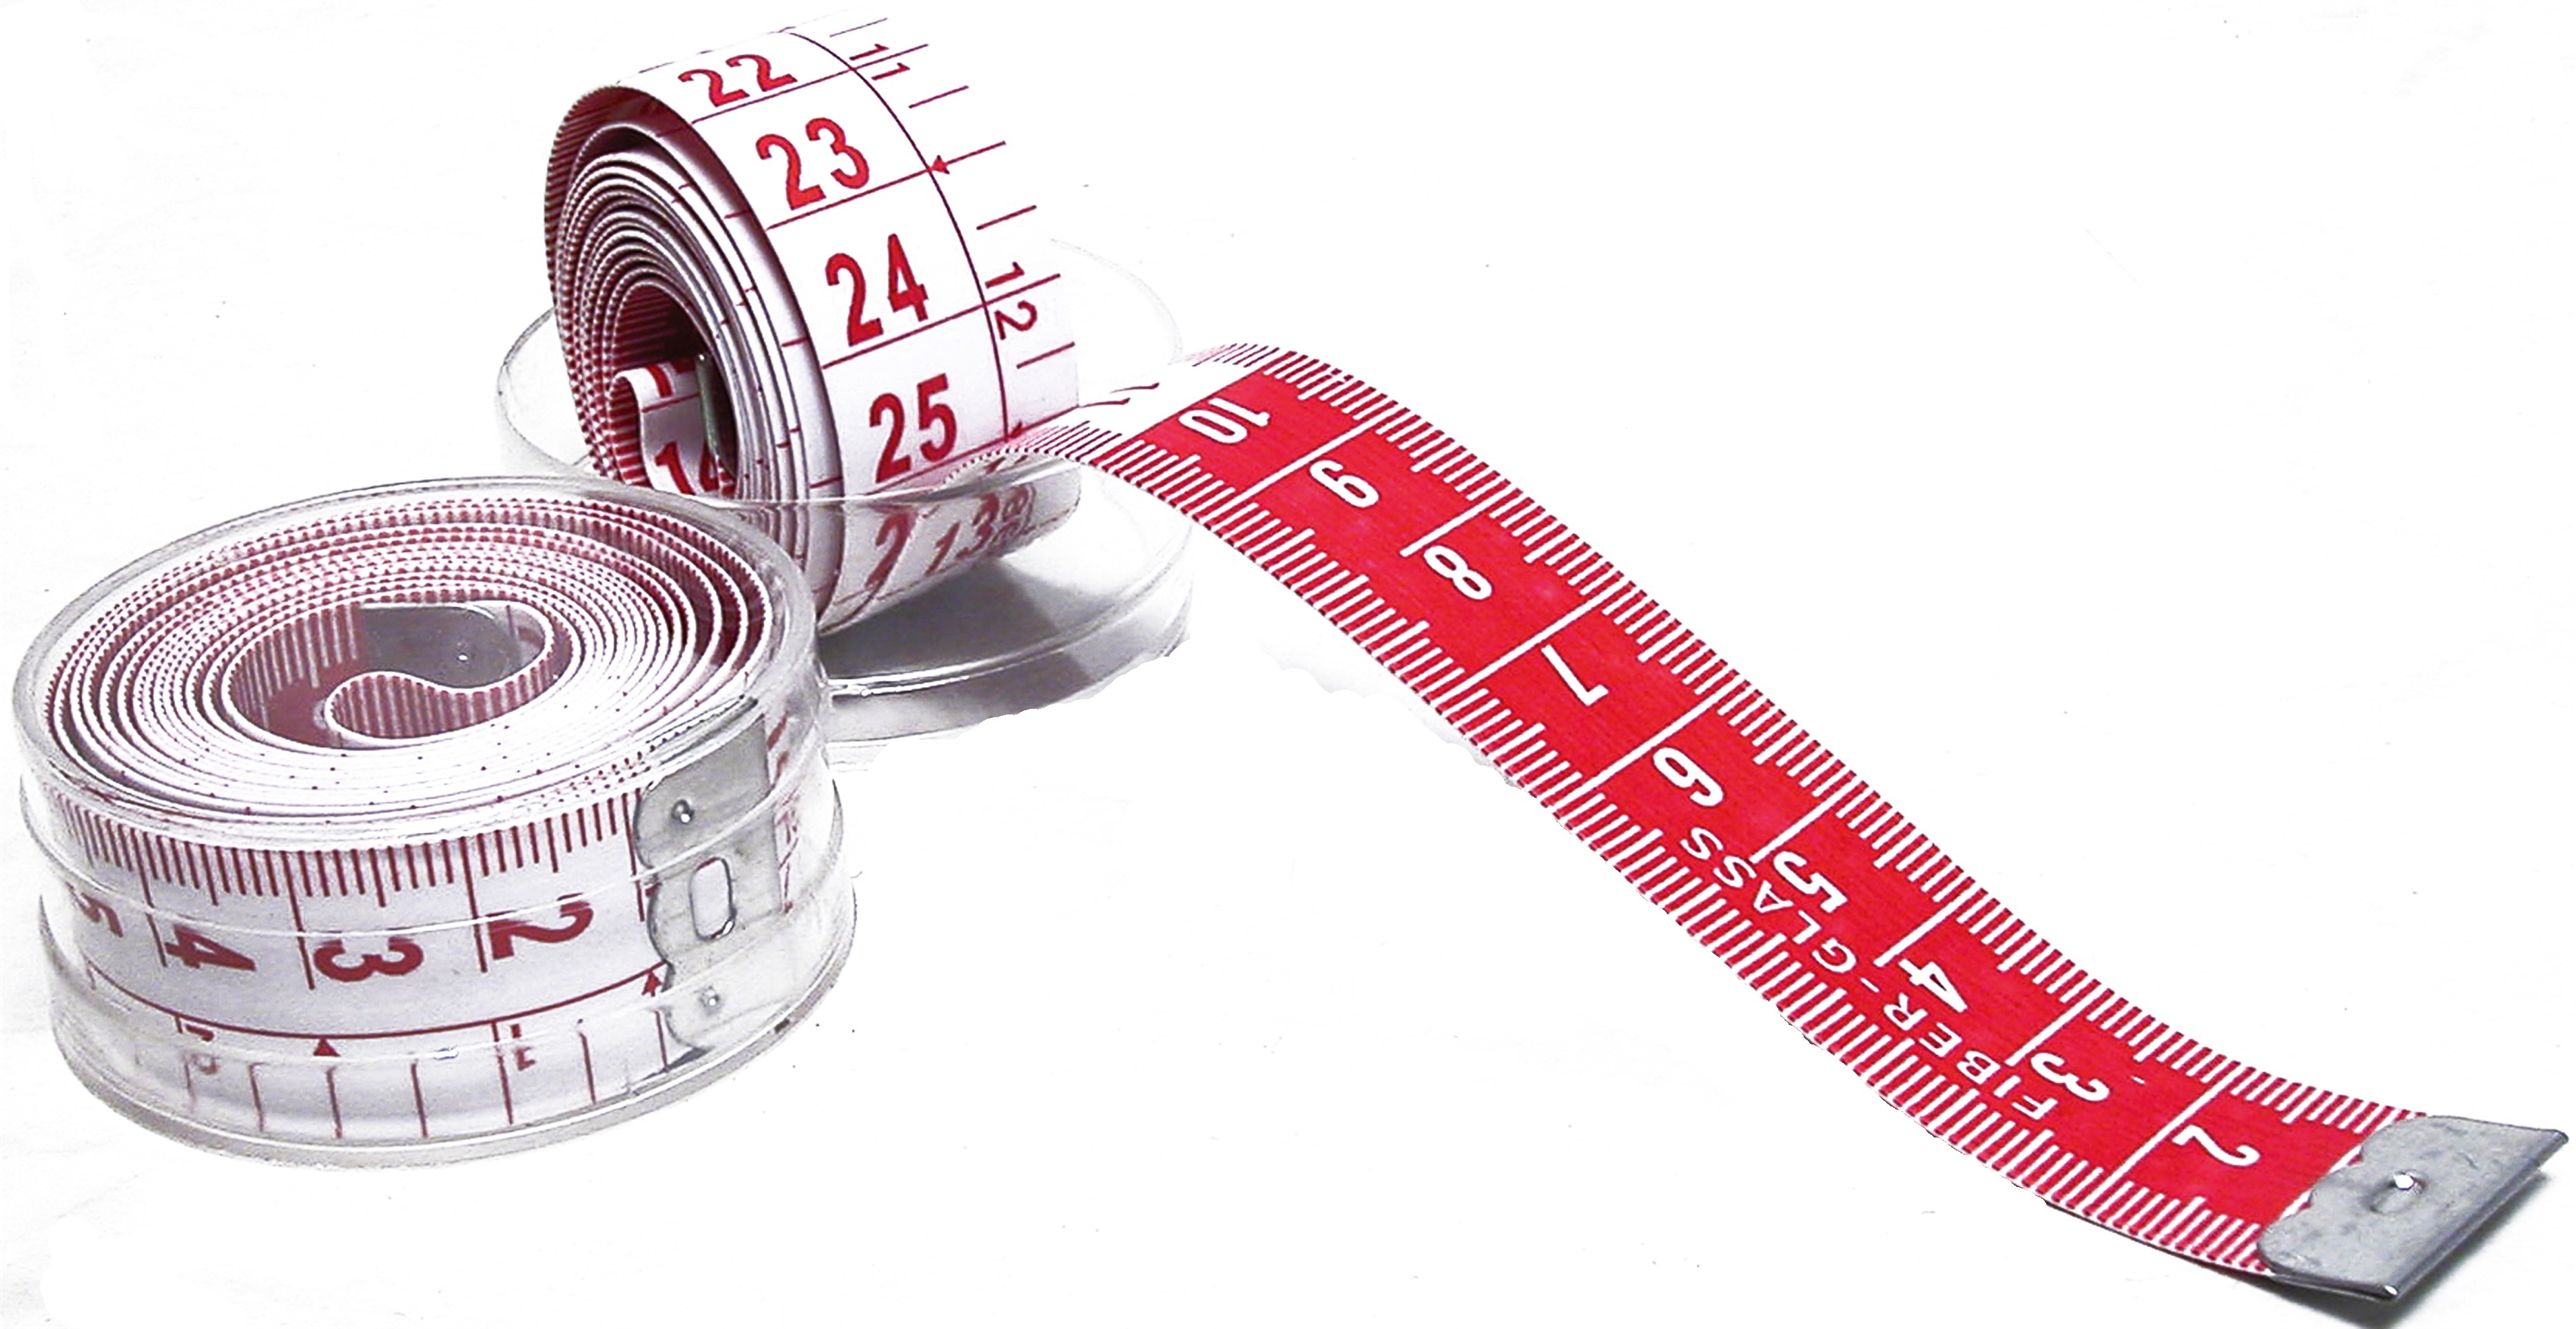
\includegraphics[height = 2in, width = 4in]{images/fit.jpeg}
   \end{center}
\end{frame}

\begin{frame}
  \frametitle{Vantagens}
   Ganho de desempenho.\\
   \begin{center}
    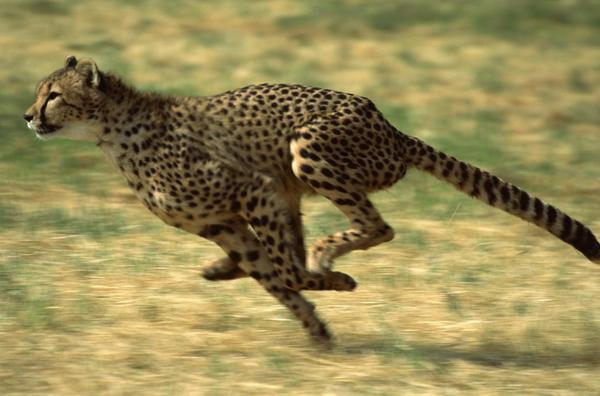
\includegraphics[height = 2in, width = 3in]{images/fast.jpeg}
   \end{center}
\end{frame}

\begin{frame}
  \frametitle{Vantagens}
   Maior segurança.\\
   \begin{center}
   
\includegraphics[height = 2in, width = 2in]{images/security.jpeg}
   \end{center}
\end{frame}

%SLIDES == EXEMPLO
\section{Pré-requisitos}

\begin{frame}
 \frametitle{Pacotes}
 \begin{center}
  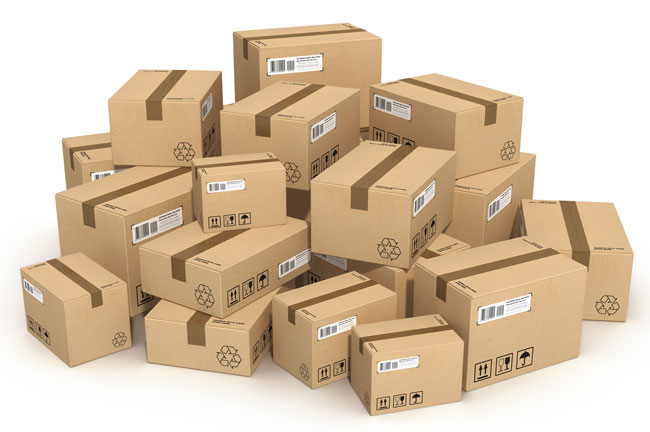
\includegraphics[height = 2in, width = 3in]{images/packages.jpg}
 \end{center}

\end{frame}

\begin{frame}
  \frametitle{Pacotes necessários}
  
  \begin{itemize}
   \item kernel-package
    \pause
   \item libncurses-dev
    \pause
   \item fakeroot
    \pause
   \item zlib1g-dev
  \end{itemize}

\end{frame}

\begin{frame}
  \frametitle{Instalar pacotes básicos}
    \textcolor{red}{
    sudo apt-get install kernel-package libncurses-dev fakeroot zlib1g-dev}

\end{frame}

\begin{frame}
  \frametitle{Baixe o Kernel e descompacte o mesmo}

   \begin{itemize}
    \item Baixe a versão do Kernel com a extenção \textit{.bz2}.
    \pause
    \item \url{www.kernel.org/}
    \pause
    \item Descompacte o Kernel\\
      \textcolor{red}{tar -jxvf linux-2.6.32.20.tar.bz2}
    \pause
    \item Crie um link simbólico.\\
      \textcolor{red}{ln -s /usr/src/linux-2.6.32.20 linux}
   \end{itemize}
\end{frame}

\section{Conhecendo sobre o seu hardware}

\begin{frame}
 \frametitle{Conhecendo o seu hardware}
 \begin{center}
  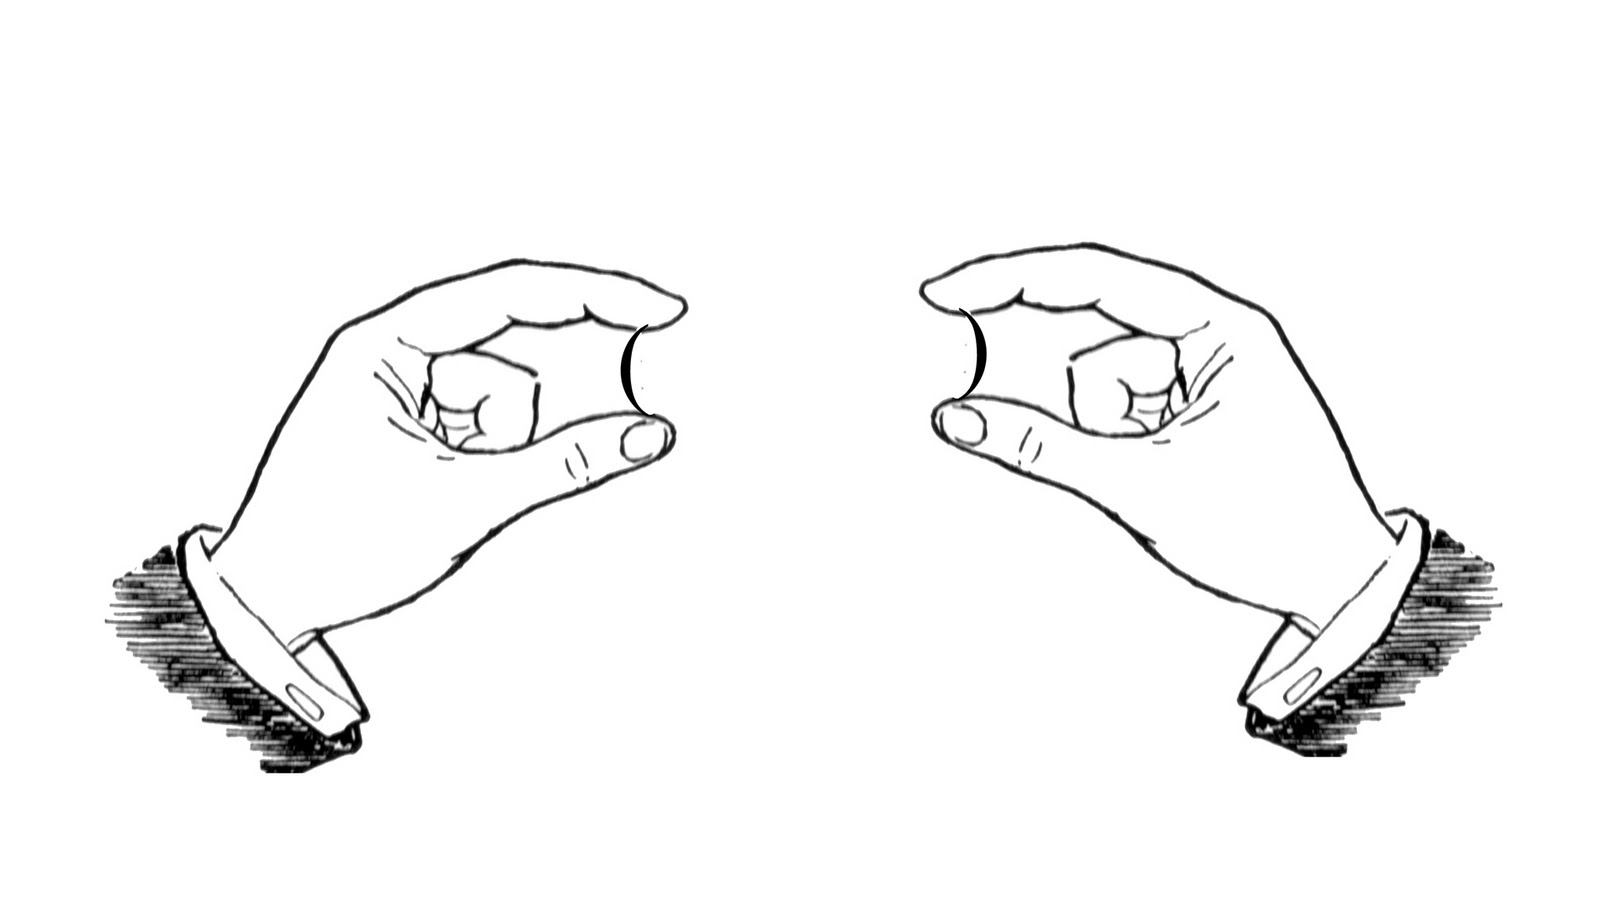
\includegraphics[height = 2in, width = 3in]{images/parenthesis.jpg}
 \end{center}

\end{frame}

\begin{frame}
  \frametitle{Conhecendo o seu hardware}
 \begin{enumerate}
  \item Mostra dados sobre o processador.\\
    \textcolor{red}{cat /proc/cpuinfo}
    \pause
  \item Exibe dispositivos PCI. \\
    \textcolor{red}{lspci -tv}
    \pause
  \item Exibe dispositivos USB. \\
    \textcolor{red}{lsusb -tv}
 \end{enumerate}

\end{frame}


\section{Menu de configuração}

\begin{frame}
 \frametitle{Arquivo e tela de configuração}
 Copiar o arquivo de configuração padrão. \\
 \begin{center}
  \textcolor{red}{cp /boot/config-`uname -r` .config} \\
 \end{center}
\end{frame}

\section{Algumas opções no menu de configuração}

\begin{frame}
  \frametitle{Configurações}
  \begin{center}
    
\includegraphics[height = 2.5in, width = 4in]{images/configuration.jpg}
  \end{center}
\end{frame}

\begin{frame}
  \frametitle{Configurações}
  \begin{center}
    \textcolor{red}{make menuconfig} \\
  \end{center}
  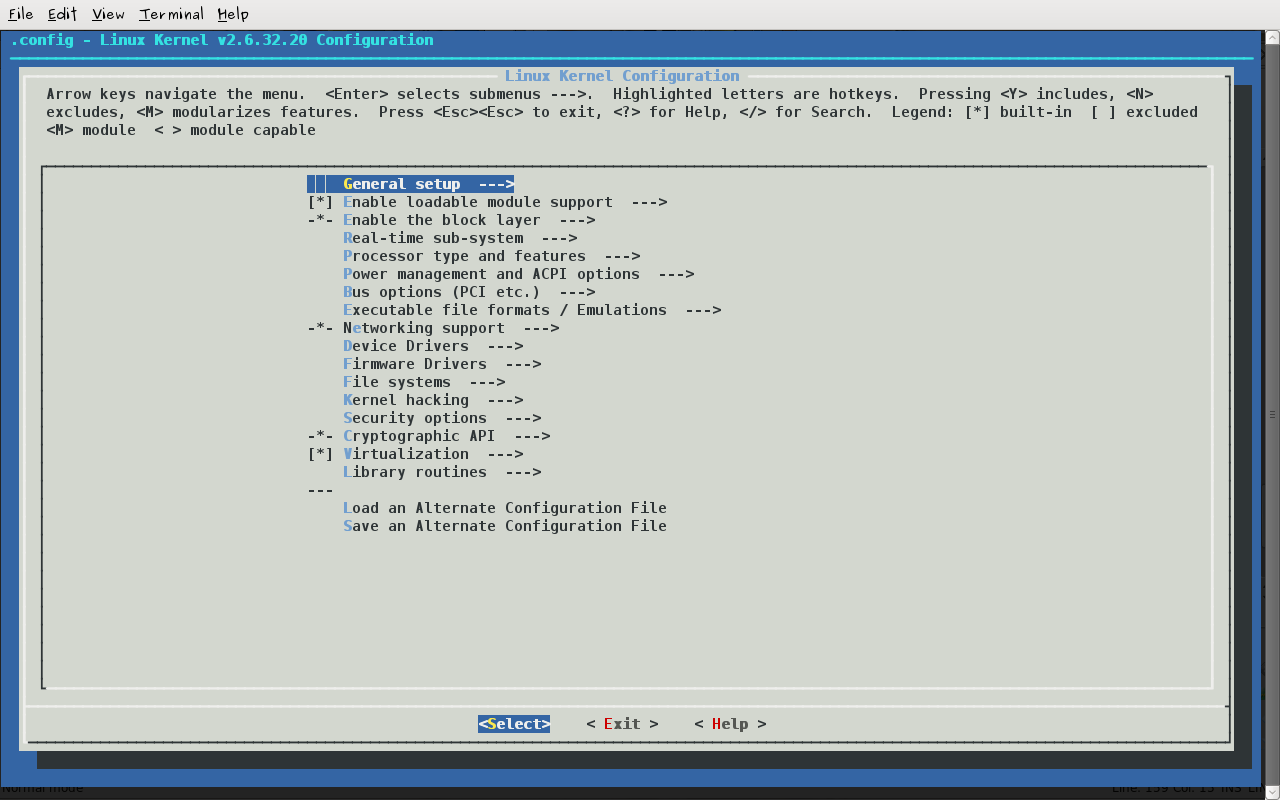
\includegraphics[height = 2.5in, width = 4in]{images/PrimeiraTela.png}
\end{frame}

\begin{frame}
 \frametitle{General Setup - Configurações gerais}
 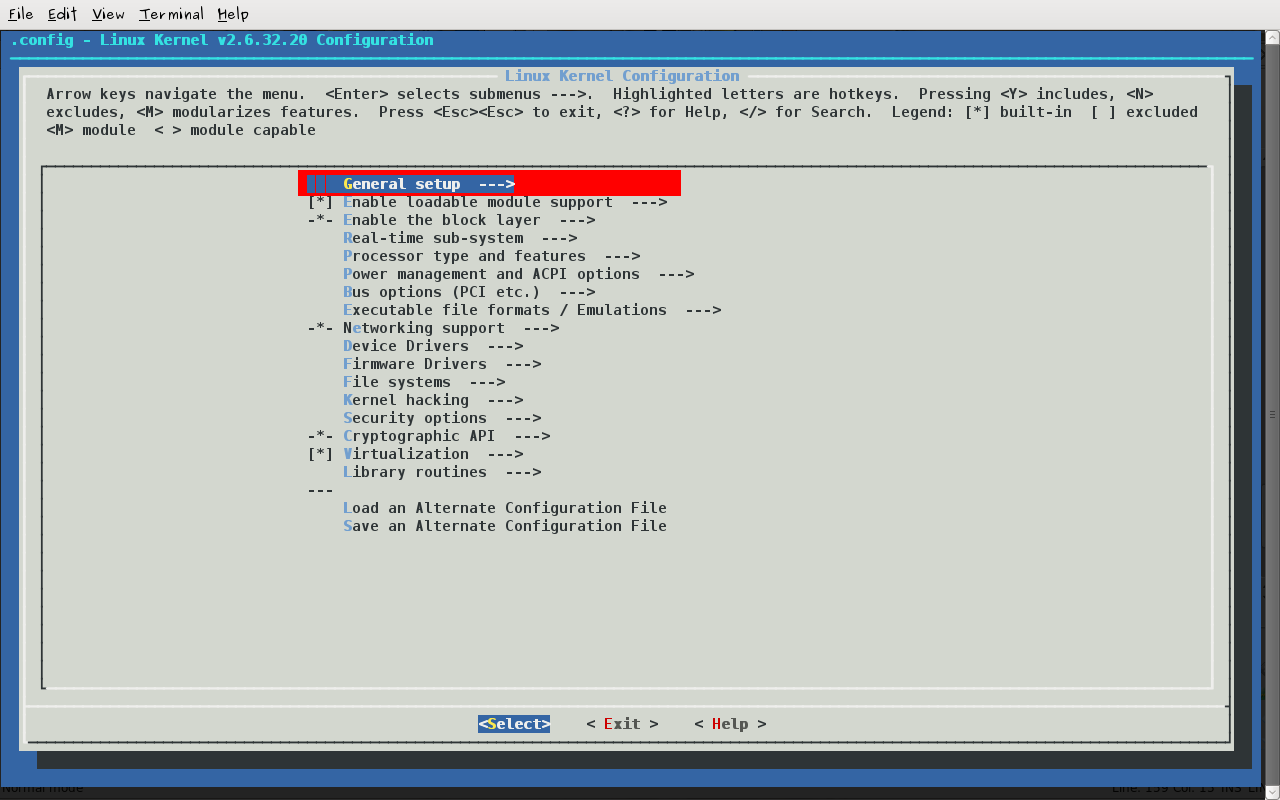
\includegraphics[height = 2.5in, width = 4in]{images/GeneralSetupInit.png}
\end{frame}

\begin{frame}
 \frametitle{General Setup - Configurações gerais}
 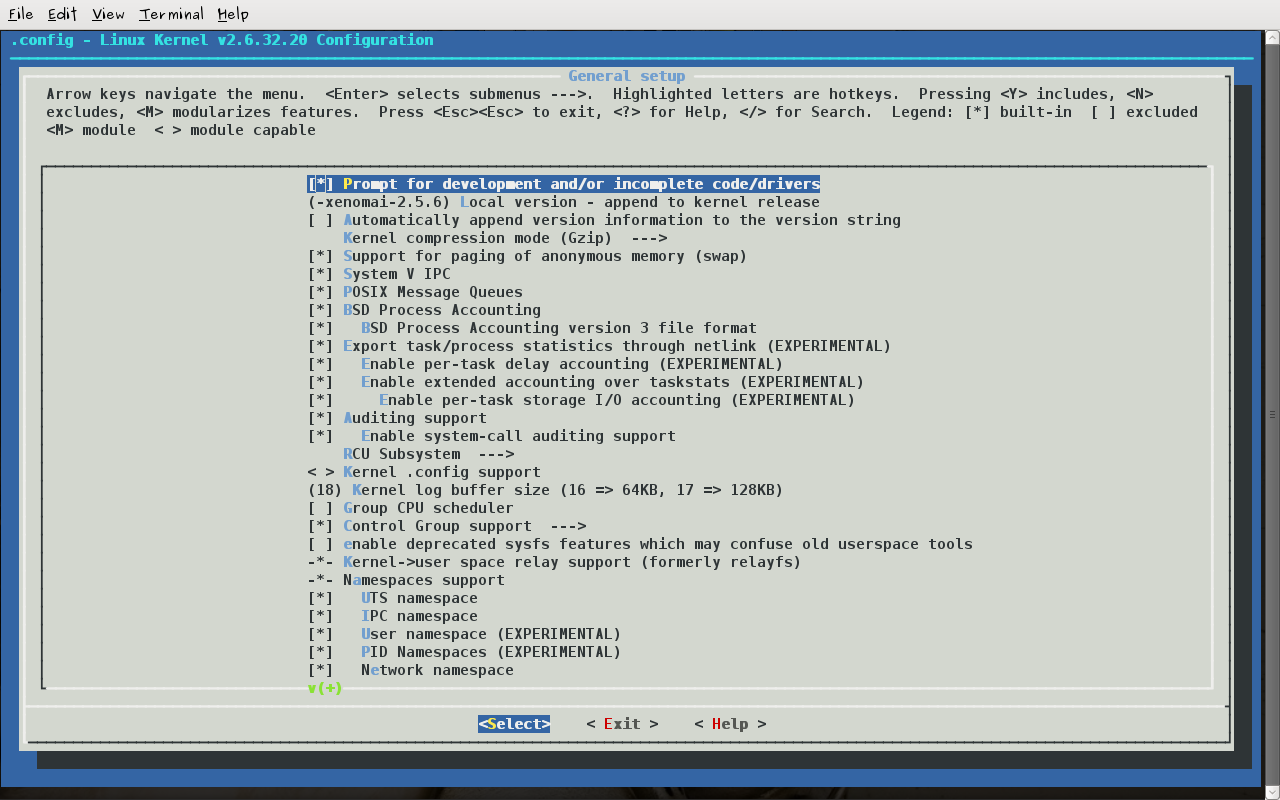
\includegraphics[height = 2.5in, width = 4in]{images/GeneralSetup1.png}
\end{frame}

\begin{frame}
 \frametitle{Enable loadable module support}
 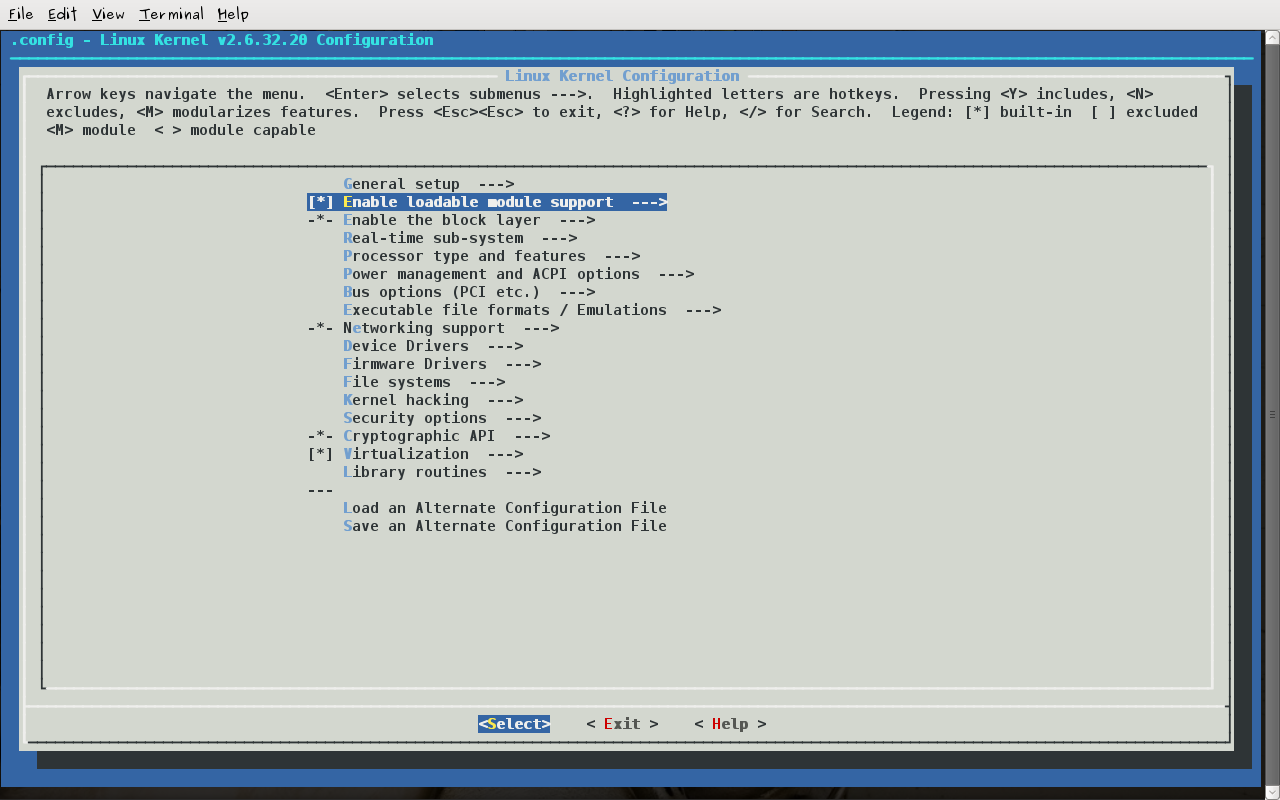
\includegraphics[height = 2.5in, width=4in]
  {images/EnableLoadableModuleSupport1.png}
\end{frame}

\begin{frame}
 \frametitle{Enable loadable module support}
 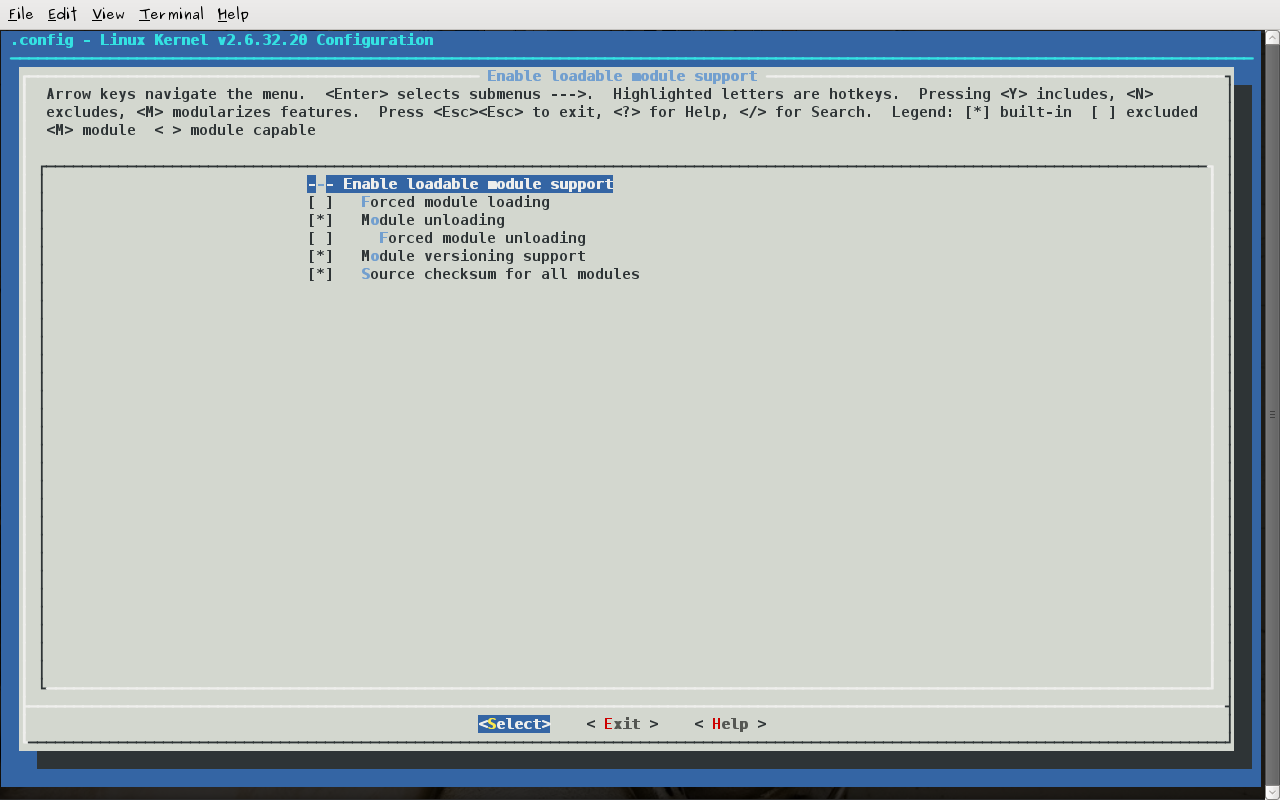
\includegraphics[height = 2.5in, width=4in]
  {images/EnableLoadableModuleSupport.png}
\end{frame}

\begin{frame}
 \frametitle{Processor type and features}
 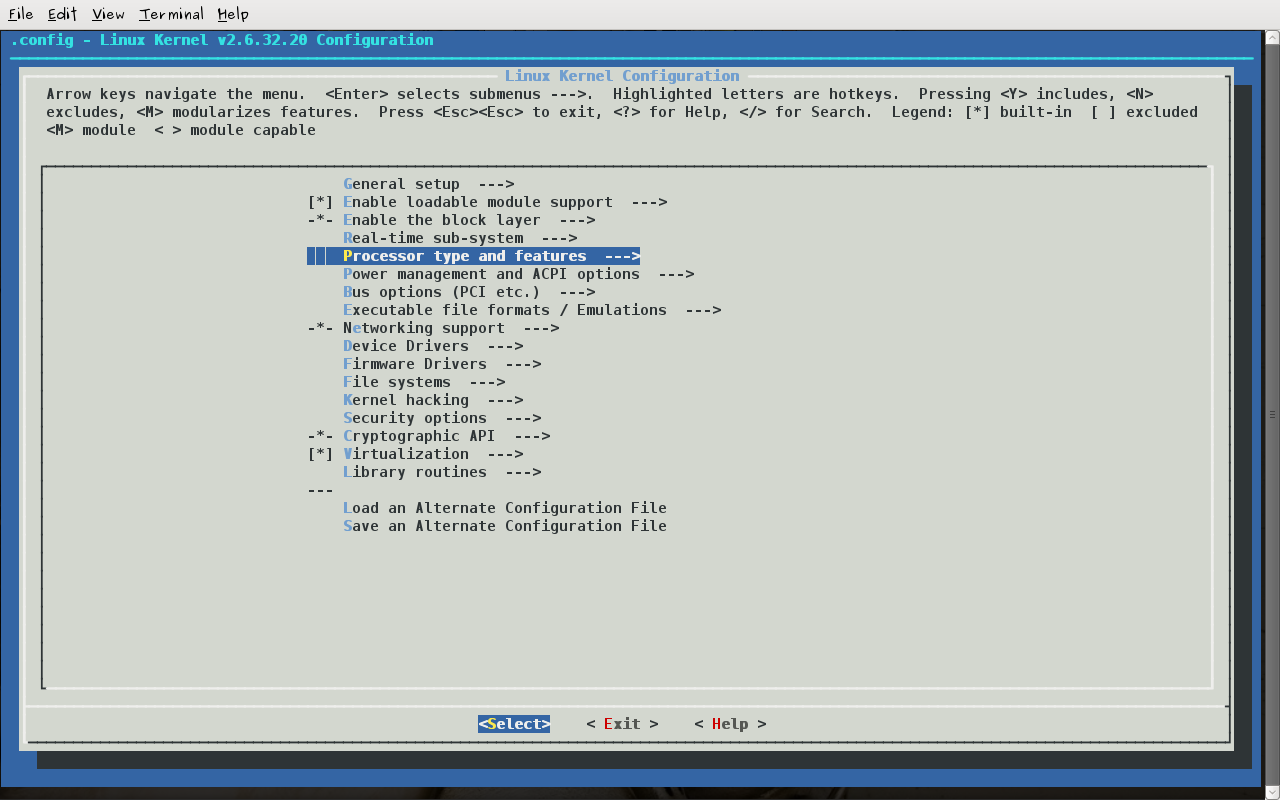
\includegraphics[height = 2.5in, width=4in]
  {images/ProcessoTypeAndFeature.png}
\end{frame}

\section{Compilando}

\begin{frame}
 \frametitle{Compile}
  \begin{center}
    
\includegraphics[height = 2in, width=2in]{images/compile.png}
  \end{center}
\end{frame}

\begin{frame}
 \frametitle{Comandos}
 Existem várias maneiras diferentes de se compilar o Kernel, seguem as duas 
  formas mais comuns:\\
  1 - \textcolor{red}{CONCURRENCY\_LEVEL=2 CLEAN\_SOURCE=no fakeroot make-kpkg 
    --initrd kernel\_image kernel\_headers}\\

  2 - \textcolor{red}{make \&\& make modules}\\
\end{frame}

\section{Instalando}

\begin{frame}
 \frametitle{Instalando o Kernel}
 Para quem utilizou o primeiro comando:\\
 \textcolor{red}{dpkg -i linux-image*.deb}
 \\
 \textcolor{red}{update-initramfs -c -k SEU\_KERNEL \&\& update-grub}
\end{frame}

\begin{frame}
 \frametitle{Instalando o Kernel}
 Para quem utilizou o segundo comando:\\
 \textcolor{red}{make modules\_install}
 \\
 \textcolor{red}{make install}
 \\
 cd boot\/
 \\
 \textcolor{red}{update-initramfs -c -K SEU\_KERNEL}
 \\
 ln -s SUA\_IMAGEM vmlinuz
 \\
 ln -s SEU\_INITRD initrd
\end{frame}


\end{document}
